\subsection{Nieuwe peiling}\label{nieuwepeiling}
In deze paragraaf zal stap voor stap beschreven worden hoe je een \emph{peiling} aanmaakt en toont op de website.

\textbf{Nieuwe peiling aanmaken}

\begin{enumerate}
\item Ga naar \drupalpath{node/add/poll}
\item Vul een vraag in bij het veld \emph{Vraag}.
\item Vul minstens twee mogelijke antwoorden in bij het veld \emph{Keuze}, klik op de knop \emph{Meer keuzes} om meerdere keuzes te specificeren.
\item Bepaal bij het veld \emph{Peilingsstatus} of de Peiling \emph{gesloten} of \emph{actief} is.
\item Selecteer hoe lang de Peiling moet duren bij het veld \emph{Peilingsduur}.
\item Specificeer optioneel een locatie bij de velden onder \emph{Locatie}.
\item Klik onderaan de pagina op de knop \emph{Opslaan} om de inhoud op te slaan.
\end{enumerate}

\begin{center}
	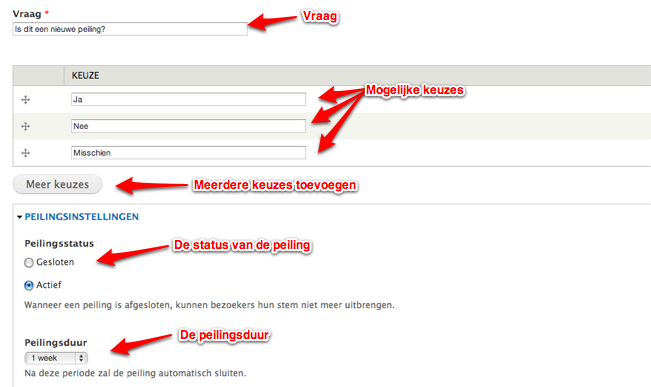
\includegraphics[width=\textwidth]{img/peiling_1.png}
\end{center}


\textbf{Nieuwe peiling tonen}

\begin{enumerate}
\item Ga naar de gewenste pagina waarop je peiling wil tonen.
\item Klik in de gewenste \emph{regio} op het \emph{tandwieltje} en klik vervolgens op \emph{Blok toevoegen}
\end{enumerate}

\begin{center}
	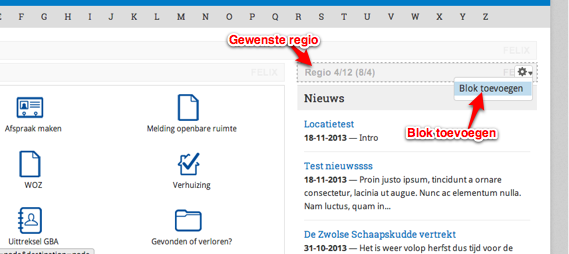
\includegraphics[width=\textwidth]{img/peiling_2.png}
\end{center}

Nadat je op het \emph{tandwieltje} hebt geklikt, zal een overzicht verschijnen welke je kunt zien in de onderstaande afbeelding.

\begin{center}
	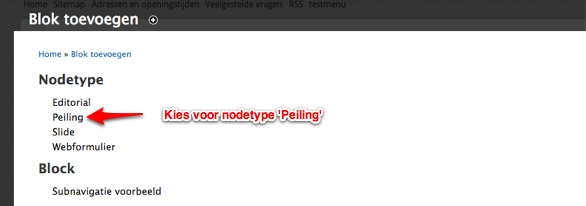
\includegraphics[width=\textwidth]{img/peiling_3.png}
\end{center}

\begin{enumerate}
\item Klik onder het kopje \emph{Nodetype} op de link genaamd \emph{Peiling}.
\item Vervolgens kun je de weergavemodus kiezen, kies voor \emph{Volledige inhoud}.
\item Nadat je op \emph{Volledige inhoud} hebt geklikt, krijg je een lijst te zien met alle bestaande peilingen, klik op de gewenste peiling. De peiling zal daarna direct toegevoegd worden aan de gewenste regio.
\item Indien je de peiling wilt verplaatsen binnen de gekozen regio, raadpleeg dan \emph{Felix blok volgorde aanpassen} \seeone{felixblokvolgorde}
\end{enumerate}

